\documentclass{beamer}

%Use the following to tell latex to NOT print navigation symbols at the bottom of each slide.
\setbeamertemplate{navigation symbols}{}

%The color of cnm
\definecolor{cnmcolor}{RGB}{0,58,112}

\usepackage{graphicx} % for including images
\usepackage{listings} %For including source code in the slides

%Change the size of the frame title.
%All sizes are listed here: https://engineering.purdue.edu/ECN/Support/KB/Docs/LaTeXChangingTheFont
\setbeamerfont{frametitle}{size=\huge}


%Global Background must be put in preamble
\usebackgroundtemplate{
%Set the background color of all pages.
%\pagecolor{cnmcolor}
%Vertical CNM color bar on left side of page.
\color{cnmcolor}\vrule width 10pt %height \paperheight
}


%Changing title font size. Courtesy of
%http://tex.stackexchange.com/questions/42136/changing-the-font-size-of-document-title
\newcommand*{\TitleFont}{%
      \usefont{\encodingdefault}{\rmdefault}{b}{n}%
      \fontsize{32}{20}%
      \selectfont}


\definecolor{MyDarkGreen}{rgb}{0.0,0.4,0.0} % This is the color used for comments
\definecolor{Blue}{rgb}{0.0,0.0,1.0}
\definecolor{Purple}{rgb}{0.4,0.0,0.4}
\lstloadlanguages{Java} % Load Java syntax for listings, for a list of other languages supported see: ftp://ftp.tex.ac.uk/tex-archive/macros/latex/contrib/listings/listings.pdf
\lstset{language=Java, % Use Java in this example
        frame=single, % Single frame around code
        basicstyle=\small\ttfamily, % Use small true type font
        keywordstyle=[1]\color{Blue}\bf, % Java functions bold and blue
        keywordstyle=[2]\color{Purple}, % Java function arguments purple
        keywordstyle=[3]\color{Blue}\underbar, % Custom functions underlined and blue
        identifierstyle=, % Nothing special about identifiers                                         
        commentstyle=\usefont{T1}{pcr}{m}{sl}\color{MyDarkGreen}\small, % Comments small dark green courier font
        stringstyle=\color{Purple}, % Strings are purple
        showstringspaces=false, % Don't put marks in string spaces
        tabsize=5, % 5 spaces per tab
        %
        % Put standard Java functions not included in the default language here
        morekeywords={rand},
        %
        % Put Java function parameters here
        morekeywords=[2]{on, off, interp},
        %
        % Put user defined functions here
        morekeywords=[3]{test},
       	%
        morecomment=[l][\color{Blue}]{...}, % Line continuation (...) like blue comment
        numbers=left, % Line numbers on left
        firstnumber=1, % Line numbers start with line 1
        numberstyle=\tiny\color{Blue}, % Line numbers are blue and small
        stepnumber=5 % Line numbers go in steps of 5
}

\begin{document}
\huge

\title{\TitleFont CS-152: Software Testing}
\author{Neal Holtschulte}
\date{\today}

\frame{\titlepage} %Welcome

\LARGE


\begin{frame}[fragile]{ Software Testing Outline}
\begin{itemize}
\item Terminology
\item Assertions and when to use them
\item Try-catch and when to use them
\item What are Exceptions
\item Further resources
\item Practice
\end{itemize}
\end{frame}


\begin{frame}[fragile]{ Terminology}

{\bf Unit testing} - testing small pieces of code (such as individual methods or functions).\\

A collection of unit tests is known as a {\bf test suite}.\\

{\bf Regression testing} is the process of repeatedly running tests.\\
\small
Source: Java An Introduction to Problem Solving and Programming by Savitch. Page 336.
\end{frame}


\begin{frame}[fragile]{ Terminology}
A {\bf test case} is an input output pair that we know to be correct. If we give our program (or a method of our program) the input and we do not get the expected output, then the program (or method) has failed the test case and we may have discovered a bug.\\

{\bf Negative test} - a test to make sure the system doesn't crash if given an unexpected input.
\end{frame}


\begin{frame}[fragile]{ Tracing}

{\bf Tracing variables} means watching the variables change value while the program is running.\\ \ \\

Often there are debugging utilities that will help you do this, but we're just going to use \emph{System.out.println}.
\end{frame}


\begin{frame}[fragile]{ Tracing}

Since we don't want all these print statements in the final version of our program we can use a 
\begin{lstlisting}
public static final boolean DEBUG = true;
\end{lstlisting}
Then you can wrap all your print statements in ifs and set DEBUG to false when you're done testing.
\begin{lstlisting}
if(DEBUG){ System.out.println("value's value is "+
          value); }
\end{lstlisting}
\end{frame}


\begin{frame}[fragile]{ Assertions}

{\bf Assertions} can be used to verify that certain conditions are true and make software more robust.

\begin{lstlisting}
/**
 * Get the largest integer value from myArray.
 */
public int getLargest(int[] myArray){
    //First check to make sure the array is 
    //not empty.
    assert(myArray.length > 0);
    ...
\end{lstlisting}
\end{frame}


\begin{frame}[fragile]{ Assertions}
\begin{itemize}
\item Assertions can and should be used throughout your code to verify that any important conditions hold.
\item Assertions provide a form of {\bf enforced documentation}.
\item Assertions help you find bugs faster.
\item Assertions do not (usually) noticeably slow down software.
\end{itemize}
\end{frame}


\begin{frame}[fragile]{ }
See TestingExample.java
\end{frame}


\begin{frame}[fragile]{ Try-catch}

{\bf Try-catch} statements can be used to throw more useful error messages or to make a program more robust by handling rare special cases.

\small
Java An Introduction to Problem Solving and Programming by Savitch. Chapter 9.
\end{frame}


\begin{frame}[fragile]{ Try-catch}
\begin{lstlisting}
public Sandwhich makePBJ(){
    PeanutButter pb;
    try{
        pb = getPB();
        if(pb.isEmpty()){
            throw new Exception("EXCEPTION: No "+
                "Peanut Butter!");
        }
    } catch (Exception e){
        System.out.println(e.getMessage());
        System.out.println("Go to the store and "+
            "buy peanut butter.");
    }
    ...
\end{lstlisting}
\end{frame}



\begin{frame}[fragile]{ Try-catch}
Try-catch blocks are required around file readers because the file might not be found.
\end{frame}


\begin{frame}[fragile]{ Try-catch}
\begin{lstlisting}
try{
    //Create a new file reader and pass it the
    //file to read in.
    FileReader fr = new FileReader("english.0");
    BufferedReader bReader = new BufferedReader(fr);
    String line = bReader.readLine();
    while(line != null){
        text += line+",";
        line = bReader.readLine();
    }
    bReader.close();
}
catch(Exception e){
    System.out.println("ERROR: There was a problem "+
        "reading the file.\n"+e.getMessage());
    System.exit(1);
}
\end{lstlisting}
\end{frame}


\begin{frame}[fragile]{ Try-catch}
Use a try-catch block whenever there is a special case that needs to be handled differently.\\ \ \\

Use a try-catch to trigger additional data-gathering when an exception occurs to help debug your code. For example:
\end{frame}


\begin{frame}[fragile]{ Try-catch}
\begin{lstlisting}
try{
    myStack.pop();
}
catch(Exception e){
    System.out.println(e.getMessage());
    myStack.printContents();
    System.exit(1);
}
\end{lstlisting}
\end{frame}


\begin{frame}[fragile]{ What are exceptions?}
\begin{itemize}
\item An exception signals an unusual event during execution.
\item Creating an exception is called ``throwing an exception".
\item Code that deals with an exception is said to ``handle an exception".
\end{itemize}
\small
Java An Introduction to Problem Solving and Programming by Savitch. Page 659.
%A divide by zero example follows, but I prefer the example starting on page 749
\end{frame}


\begin{frame}[fragile]{ What are exceptions?}
Exceptions are objects that can be created and thrown
\begin{lstlisting}
throw new Exception("EXCEPTION: No Peanut Butter!");
\end{lstlisting}
You can see what methods are available to be called on exceptions with Eclipse's autocomplete feature.
\end{frame}


\begin{frame}[fragile]{ Testing advice}
\begin{itemize}
\item Automated your testing process
\item Make test output self-identifying
\item Make tests reproducible
\item Add a test for each bug
\item Add tests for new features and changes
\item Never throw away a test
\end{itemize}
\normalsize
Further information about the above advice can be found here: \url{http://www.cs.princeton.edu/~bwk/testing.html}
\end{frame}


\begin{frame}[fragile]{ Further resources}
\begin{itemize}
\item Software Testing (free online course) \normalsize \url{https://www.udacity.com/course/cs258} \LARGE
\item Java Exceptions tutorial \normalsize \url{http://docs.oracle.com/javase/tutorial/essential/exceptions/definition.html} \LARGE
\end{itemize}
\end{frame}


\begin{frame}[fragile]{ Software Testing Outline}
\begin{itemize}
\item Terminology
\item Assertions and when to use them
\item Try-catch and when to use it
\item What are Exceptions
\item Further resources
\item Practice
\end{itemize}
\end{frame}


\begin{frame}[fragile]{ Before we practice, Stacks}
%http://ttuxen.wordpress.com/2011/02/21/embedding-lua-in-c-net-part-iii/
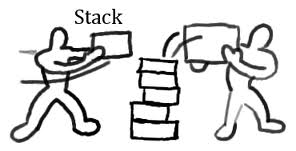
\includegraphics[scale=1.0]{images/stack.jpg}
\end{frame}


\begin{frame}[fragile]{ }
%http://brendan.enrick.com/post/understanding-the-stack-data-structure.aspx
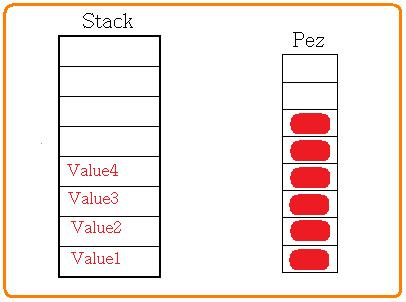
\includegraphics[scale=1.0]{images/pez.jpg}
\end{frame}


\begin{frame}[fragile]{ }
%http://www.cs.auckland.ac.nz/software/AlgAnim/stacks.html
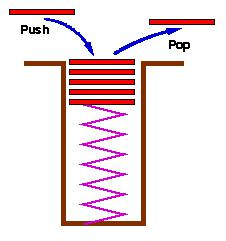
\includegraphics[scale=1.0]{images/stack1.jpg}
\end{frame}


\begin{frame}[fragile]{ Let's ...}
\begin{itemize}
\item look at the stack code
  \begin{itemize}
  \item where might we insert assertions?
  \item what can go wrong?
  \end{itemize}
\item test the constructor
\item discuss if negative tests are reasonable
  \begin{itemize}
  \item use an assertion
  \item use a try-catch
  \end{itemize}
\item divide up and write tests for the buggy stack implementations
\end{itemize}
\end{frame}


\begin{frame}[fragile]{ Let's ...}
To Eclipse.\\ \ \\

code/StackTestingCode/
\end{frame}


\end{document}